\chapter{Conditionnement du signal}
\subsubsection{Introduction}
L'information électronique peut se trouver sur beaucoup de forme (tension, courant, charge électrique, impédance ou variation d'impédance). Mais beaucoup de dispositifs de mesure ne traitent que des signaux électriques sous forme de tension, dans une gamme de valeur déterminée. Pour reménédier à cela, nous avons besoin d'un conditionneur
\begin{description}
	\item[conditionneur] montage électronique qui transforme la grandeur de sortie du transducteur en tension (si nécessaire) et l'amplifie
\end{description}
Il peut aussi corriger les problèmes de linéarité de la caractéristique du transducteur et de compensation des grandeurs d'influence.
\subsubsection{Principes fondamentaux de mesure}
Il existe 2 principes de base:
\begin{enumerate}
	\item méthode de déflexion: mesurer la valeur absolue d'une grandeur (mesure classique)
	\item méthode de zéro: compenser la valeur absolue d'une grandeur par des valeurs étalonnées connues, plus robuste aux parasites (comparaison) mais plus lent (itératif)
\end{enumerate}
On peut aussi avoir un signal fréquentiel car:
\begin{itemize}
	\item il est insensible aux parasites
	\item convient bien pour les longues distances
	\item avec une conversion A/N aisée par comptage de périodes
	\item à des références de fréquences très précises
\end{itemize}
on convertit en fréquence grâce à un oscillateur LC dont l'une des 2 impédances est le capteur. On peut détecter le signal par
\begin{itemize}
	\item mesure direct de la fréquence (valeur absolue)
	\item battement avec un oscillateur de référence (valeur relative, plus souvent)
\end{itemize}
\section{Conversion du signal}
\subsection{Transducteur délivrant un courant}
Le conditionneur est un convertisseur courant/tension.
\begin{figure}[H] 
	\centering 
	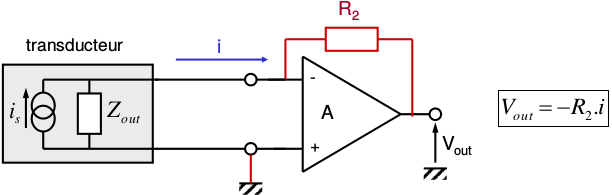
\includegraphics[width=0.7\textwidth,height=10\baselineskip,keepaspectratio]{ch4/image4} 
	\caption{Convertisseur courant/tension} 
\end{figure}
Par le zéro virtuel, il n'y a pas de courant dans \(Z_{out}\), donc le résultat est peu sensible à l'impédance de sortie du transducteur. Par contre, si courant faible (\si{\nano\ampere}), il faut \(R_2\gg\) (bonjour l'encombrement et le bruit de fond). Il faut aussi faire gaffe aux courants de polarisation de l'AOP (CN: \(i_{pol}\ll i)\)
\subsection{Transducteur délivrant une charge électrique}
Le conditionneur est un convertisseur charge/tension.
\begin{figure}[H] 
	\centering 
	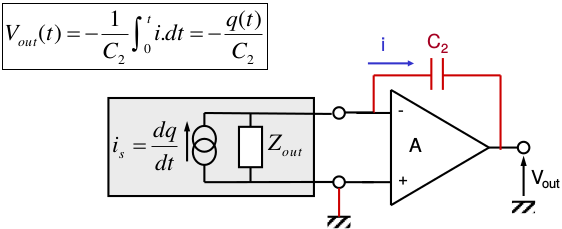
\includegraphics[width=0.6\textwidth,height=10\baselineskip,keepaspectratio]{ch4/image5} 
	\caption{Convertisseur charge/tension} 
\end{figure}
En pratique, il faut une résistance en \(\parallelsum\) sur \(C_2\) pour permettre la circulation du courant de polarisation de l'AOP \(\Rightarrow\) comportement type passe-haut.
\subsection{Transducteur résistif (résistance absolue)}
Mesure de résistance "4 fils" : permet la mesure précise de résistance de faible valeur.
\begin{figure}[H] 
	\centering 
	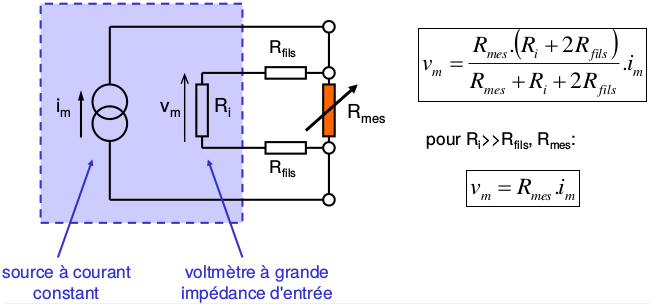
\includegraphics[width=0.8\textwidth,height=10\baselineskip,keepaspectratio]{ch4/image6} 
	\caption{Mesure de résistance 4 fils} 
\end{figure}
\subsection{Transducteur résistif (variation de résistance): Pont de Wheatstone}
	\begin{itemize}
		\item Méthode de déflection:
		\begin{itemize}
			\item mesure la différence de tension apparaissant dans la branche diagonale suite à la variation de résistance d'une des branches du pont
			\item nécessite une source de tension stable
		\end{itemize}
		\item Méthode du zéro
		\begin{itemize}
			\item annulation de la f.e.m. précédente par variation d'une seconde résistance calibrée
			\item nécessite PAS d'une source de tension stable
			\item plus lent
		\end{itemize}
	\end{itemize}
\subsubsection{1 résistance variable}
\begin{minipage}[t]{0.8\textwidth}
	\begin{itemize}
		\item hypothèses:
		\begin{itemize}
			\item Impédance de source négligeable
			\item Impédance du voltmètre très élevée
		\end{itemize}
	\end{itemize}
	\[v_{ab} = \left(\frac{R_4}{R_1+R_4}-\frac{R_3}{R_2+R_3}\right)E\]
	la variation de \(R_1\) étant faible (max \SI{1}{\percent}), on linéarise
	\begin{align*}
		\Delta v_{ab} &= \frac{\partial v_{ab}}{\partial R_1}\Delta R_1\\
		&= -E\frac{R_4}{(R_1+R_4)^2}\Delta R_1
	\end{align*}
	Si les 4 résistances sont identiques:
	\[\Delta v_{ab} = -\frac{E}{4}\frac{\Delta R}{R}\]
	Pour augmenter la sensibilité, \(\nearrow E\), mais limité par le courant max (10\textasciitilde100 \si{\milli\ampere} max)
\end{minipage}\begin{minipage}[t]{0.2\textwidth}
\begin{figure}[H] 
	\centering 
	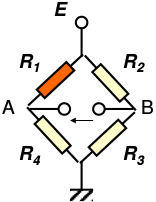
\includegraphics[width=0.8\textwidth,height=10\baselineskip,keepaspectratio]{ch4/image7} 
	\caption{Pont de Wheatstone: 1 résistance variable} 
\end{figure}
\end{minipage}
\subsubsection{montage "push-pull" (2 résistances)}
\begin{figure}[H] 
	\centering 
	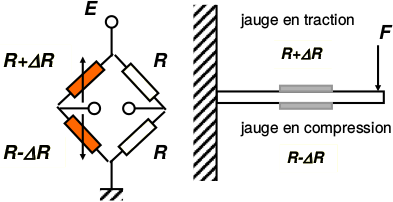
\includegraphics[width=0.5\textwidth,height=7\baselineskip,keepaspectratio]{ch4/image8} 
	\caption{Pont de Wheatstone: "push-pull" (2 résistance variable)} 
\end{figure}
	le capteur impose des variations = et >< aux 2 résistances variables. Ceci renforce les différences, doublant la sensibilité
	\[\Delta v_{ab}=-\frac{E}{2}\frac{\Delta R}{R}\]
\subsubsection{4 résistances variables}
\begin{figure}[H] 
	\centering 
	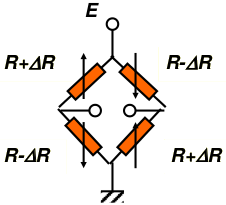
\includegraphics[width=0.8\textwidth,height=7\baselineskip,keepaspectratio]{ch4/image9} 
	\caption{Pont de Wheatstone: 4 résistances variables} 
\end{figure}
	Sensibilité encore doublé (donc quadruplé au total)
	\[\Delta v_{ab}=-E\frac{\Delta R}{R}\]

\subsubsection{Mesure "3 fils"}
\begin{minipage}[t]{0.6\textwidth}
	Autre application du montage à 2 résistances variables, il élimine l'influence des variations de résistance des fils de connexion au capteur (soustraction des variations des 2 branches de gauche). Il possède la même sensibilité que le pont de Wheatstone à \textbf{1 seule} résistance variable
	\[\Delta v_{ab} = -\frac{E}{4}\frac{\Delta R}{R}\]
\end{minipage}\begin{minipage}[t]{0.4\textwidth}
\begin{figure}[H] 
	\centering 
	\vspace{-2.3cm}
	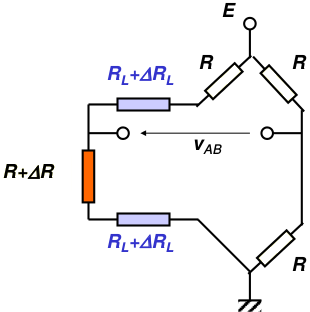
\includegraphics[width=0.8\textwidth,height=10\baselineskip,keepaspectratio]{ch4/image10} 
	\caption{Pont de Wheatstone: mesure "3 fils"} 
\end{figure}
\end{minipage}
\subsection{Transducteur réactif (pont d'impédance)}
\begin{minipage}[t]{0.8\textwidth}
	Généralisation du pont de Wheatstone avec \(Z_1, Z_2=\) réactances, sous principe du "push-pull" avec la linéarité et une meilleure sensibilité. Par contre, l'alim. doit être en alternatif (typiquement quelques \si{\kilo\hertz})
\end{minipage}\begin{minipage}[t]{0.2\textwidth}
\begin{figure}[H] 
	\centering 
	\vspace{-2.1cm}
	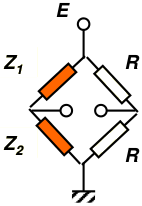
\includegraphics[width=0.8\textwidth,height=7\baselineskip,keepaspectratio]{ch4/image11} 
	\caption{Pont d'impédance} 
\end{figure}
\end{minipage}
\section{Amplification}
\subsection{Introduction}
Il y a 4 bonnes raisons d'amplifier:
\begin{enumerate}
	\item Protection vis-à-vis des parasites augmentant le niveau relatif du signal (amplifier le plus près du transducteur, pré-ampli grand gain / faible bruit)
	\item Précision de la conversion analogique/numérique (perte de précision si le signal ne couvre pas toute la gamme de tension d'entrée du CAN, amplification à gain variable)
	\item réjection des parasites de mode commun (amplification différentielle)
	\item adaptation d'impédance (le plus souvent réalisable au niveau de l'ampli)
\end{enumerate}
\subsection{Montages et composants amplificateurs}
Généralement, on veut:
\begin{itemize}
	\item Pré-ampli à gain élevé et faible bruit (souvent étages d'entrée à transistors discrets)
	\item ampli différentiel:
	\begin{itemize}
		\item entrée différentiel
		\item gain variable
		\item CMRR élevé
		\item symétrie des entrée
		\item supporte tension de mode commun élevée
	\end{itemize}
\end{itemize}
\subsubsection{Montage à 1 ampli-op}
\begin{minipage}[t]{0.55\textwidth}
	Le schéma de base est un montage à 4 résistances:
	\begin{itemize}
		\item rétroaction sur la branche (-)
		\item diviseur sur la branche (+)
	\end{itemize}
	Le signal différentiel est amplifié d'un gain fixe et le signal mc est amplifié d'une petite valeur (voir nulle).
\end{minipage}
\begin{minipage}[t]{.45\textwidth}
	\vspace{-2cm}
	\begin{figure}[H]
		\centering
		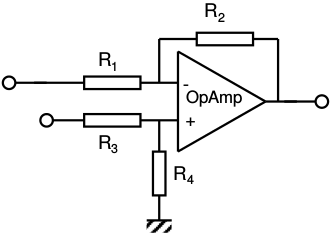
\includegraphics[width=0.7\textwidth,height=10\baselineskip,keepaspectratio]{ch4/image1} 
		\caption{montage à un seul ampli-op} 
	\end{figure}
\end{minipage}
\[G_d = \frac{R_1+R_2}{2R_1}\left(\frac{R_4}{R_3+R_4}+\frac{R_2}{R_1+R_2}\right)\qquad G_{mc}=\frac{R_1R_4-R_2R_3}{R_1(R_3+R_4)}\]
\begin{proof}
	\[V_{out} = V_{in^+}\frac{R_4}{R_3+R_4}\frac{R_2+R_1}{R_1}-V_{in^-}\frac{R_2}{R_1}\]
	Pour le mode commun, par définition \(V_{in^+} = V_{in^-} = V_{cm}\), donc
	\[V_{out} = V_{cm}\frac{R_4}{R_3+R_4}\frac{R_2+R_1}{R_1}-V_{cm}\frac{R_2}{R_1}\]
	\begin{align*}
		G_{cm}=\frac{V_{out}}{V_{cm}} &= \frac{R_4}{R_3+R_4}\frac{R_2+R_1}{R_1}-\frac{R_2}{R_1}\\
		&= \frac{R_1R_4-R_2R_3}{R_1(R_3+R_4)}
	\end{align*}
	Pour le mode différentiel, par définition \(V_{in^+} = -V_{in^-}=\frac{V_{dm}}{2}\), donc
	\[V_{out} = \frac{V_{dm}}{2}\frac{R_4}{R_3+R_4}\frac{R_2+R_1}{R_1}+\frac{V_{dm}}{2}\frac{R_2}{R_1}\]
	\begin{align*}
		G_{d} = \frac{V_{out}}{V_{dm}} &= \frac{1}{2}\frac{R_4}{R_3+R_4}\frac{R_2+R_1}{R_1} + \frac{1}{2}\frac{R_2}{R_1}\\
		&= \frac{R_1+R_2}{2R_1}\left(\frac{R_4}{R_3+R_4}+\frac{R_2}{R_1+R_2}\right)
	\end{align*} 
\end{proof}
On peut théoriquement annuler \(G_{mc}\) si \[\frac{R_2}{R_1}=\frac{R_4}{R_3}\Rightarrow G_d=\frac{R_2}{R_1}\]. En pratique \(R_1=R_3\text{ et }R_2=R_4\) mais ce n'est jamais réellement satisfait à cause des tolérances sur les résistances.\\
Les résistance de source doivent être incluse dans \(R_1\text{ et }R_3\).
\begin{description}
	\item[inconvénients] faible impédance d'entrée (gain va dépendre des résistances de source du montage en amont) et difficile de réaliser un gain variable
\end{description}
\subsubsection{Montage à 2 ampli-op}
\begin{figure}[H] 
	\centering 
	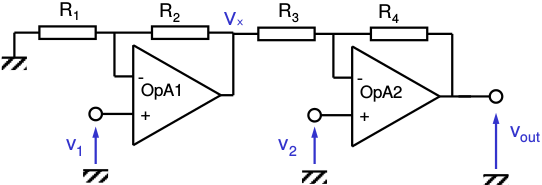
\includegraphics[width=0.55\textwidth,height=10\baselineskip,keepaspectratio]{ch4/image2} 
	\caption{Montage à 2 ampli-op} 
\end{figure}
\[G_d = \frac{1}{2}\left[1+\frac{R_4}{R_3}\left(2+\frac{R_2}{R_1}\right)\right]\qquad G_{mc} = \frac{R_1R_3-R_2R_4}{R_1R_3}\]
\begin{proof}
	\[V_x = \frac{R_1+R_2}{R_1}V_1\]
	\[\Rightarrow V_{out} = -\frac{R_4}{R_3}\frac{R_1+R_2}{R_1}V_1+\frac{R_3+R_4}{R_3}V_2\]
	pour le mode commun \(V_1=V_2=V_{mc}\)
	\begin{align*}
		G_{mc} = \frac{V_{out}}{V_{mc}} &=\frac{R_1R_3+R_1R_4-R_1R_4-R_2R_4}{R_1R_3}\\
		&= 1-\frac{R_2R_4}{R_1R_3}
	\end{align*}
	pour le mode différentiel \(V_1=-V_2=\frac{V_d}{2}\)
	\begin{align*}
		G_d=\frac{V_{out}}{V_d} &= \frac{1}{2}\left(1+\frac{R_4}{R_3}+\frac{R_4}{R_3}\frac{R_1+R_2}{R_1}\right)\\
		&= \frac{1}{2}\left[1+\frac{R_4}{R_3}\left(2+\frac{R_2}{R_1}\right)\right]
	\end{align*}
\end{proof}
De nouveau, on peut annuler \(G_{mc}\) si 
\[\frac{R_1}{R_2}=\frac{R_4}{R_3}\Rightarrow G_d = 1+\frac{R_1}{R_2}\]
\begin{itemize}
	\item \textbf{avantages}:
	\begin{itemize}
		\item impédances d'entrée élevées (celle de AOP) \(\Rightarrow\) gains indépendants des impédances de source
	\end{itemize} 
	\item \textbf{inconvénients}:
	\begin{itemize}
		\item si \(v_{cm}\) élevée et \(G_d\) faible \(\rightarrow\) risque de saturation du 1\up{er} étage
		\item les parcours des signaux (+) et (-) ne sont pas identiques, de sorte que la réponse en fréquence n'est pas la même pour les deux signaux
		\item par chaque valeur du gain, il faut apparier \(2\times 2\) résistances
	\end{itemize}
\end{itemize}
\subsubsection{Ampli d'instrumentation (3 ampli-op)}
\begin{figure}[H] 
	\centering 
	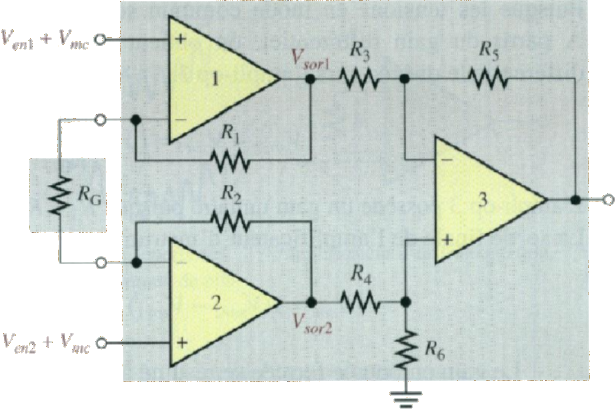
\includegraphics[width=0.8\textwidth,height=10\baselineskip,keepaspectratio]{ch4/image3} 
	\caption{Ampli d'instrumentation} 
\end{figure}
C'est la solution standard. Chaque voie passe par un AOP monté en non-inverseur, le 3\up{ème} AOP réalise la différence entre les deux signaux.
\begin{itemize}
	\item \textbf{atouts}:
	\begin{itemize}
		\item Impédance d'entrée élevée
		\item CMRR \num{90} à \SI{120}{\decibel}
		\item symétrie des deux voies
		\item résistance de réglage externe (\(R_G\)) pour faire varier le gain sans dégrader le CMRR
		\item Le potentiel au milieu de \(R_G = v_{mc}\Rightarrow\) peut être utiliser pour circuit de garde
	\end{itemize}
	\item \textbf{limitation}:
	\begin{itemize}
		\item ça va pas si \(v_{mc}\) dépasse \SI{70}{\percent} des tensions d'alim.
	\end{itemize}
\end{itemize}
\subsubsection{Ampli d'isolation}
\textit{C.f} \autoref{subsec:montdiffvmcgrand} (2 bornes de masse, 1 avant l'isolation, 1 après). On l'utilise quand \(v_{mc}\) est trop grand pour utiliser un ampli d'instrumentation. C-à-d que soit le signal différentiel est très faible sur la tension de mode commun \(>\SI{70}{\percent}\) de l'alim., soit la différence de tension entre les masses présente un danger.
\subsubsection{Imperfections des ampli-op}
2 cas:
\paragraph{Décalage statique} 2 origines: le déséquilibre des voies inverseuse et non-inverseuse (\(\Rightarrow\) ampli. de précision) et les courants de polarisation (courant d'entrée de AOP). Ces grandeurs varient avec la température et la tension d'alim. On peut essayer de compenser le décalage globale manuellement ou automatiquement (autozéro)
\paragraph{Caractéristique dynamique} la bande passante et le slew-rate (pente max. qu'un AOP peut délivrer).
